\htwo{API-Architektur}
\sectionauthor{Johannes Polzer}
% todo: eventuell einzelne Punkte genauer ausformulieren

Um den Servercode besser zu strukturieren wurde ein spezieller Wrapper von ExpressJs entwickelt. Diese Grundstruktur erlaubt es, alle Endpunkte in einzelnen sogenannten "Controller"-Klassen zu implementiert. Die Architektur der API besteht aus einigen Verzeichnissen, welche in der Abbildung \ref{fig:apiStructure} dargestellt werden. Um diesen Wrapper zu nutzen, muss eine Instanz der "App"-Klasse erstellt werden.

\begin{figure}[H]
    \centering
    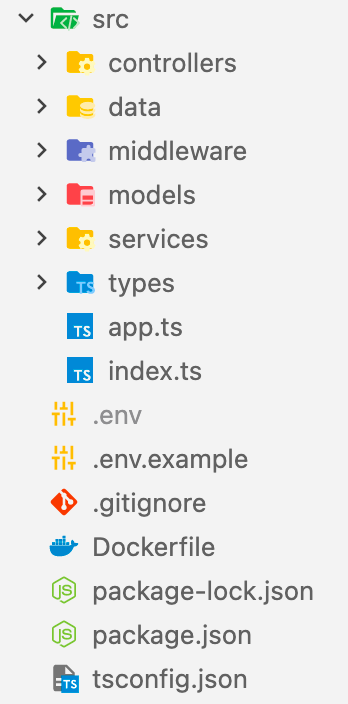
\includegraphics{media/APITemplate/ProjectStructure.png}
    \caption{Projektstruktur}
    \label{fig:apiStructure}
\end{figure}

\pagebreak
\hthree{Die "App"-Klasse}\label{sec:app}

Die "App"-Klasse übernimmt die Verwaltung aller Endpunkte, und damit das Routing zu den verfügbaren Pfaden der URL.
Das bedeutet, dass hier alle Pfade definiert werden müssen. 
Ein Pfad wird dabei durch eine sogenannte "Controller" Klasse abgebildet (siehe Kapitel \ref{sec:controller} auf Seite \pageref{sec:controller}). 
Wenn ein Request an die API gestellt wird, wird mit Hilfe des NPM-Moduls "express" die passende "Handler"-Methode des jeweiligen "Controllers" aufgerufen. 
Diese Methode bearbeitet die Anfrage und sendet eine Antwort zurück.

\begin{figure}[H]
    \centering
    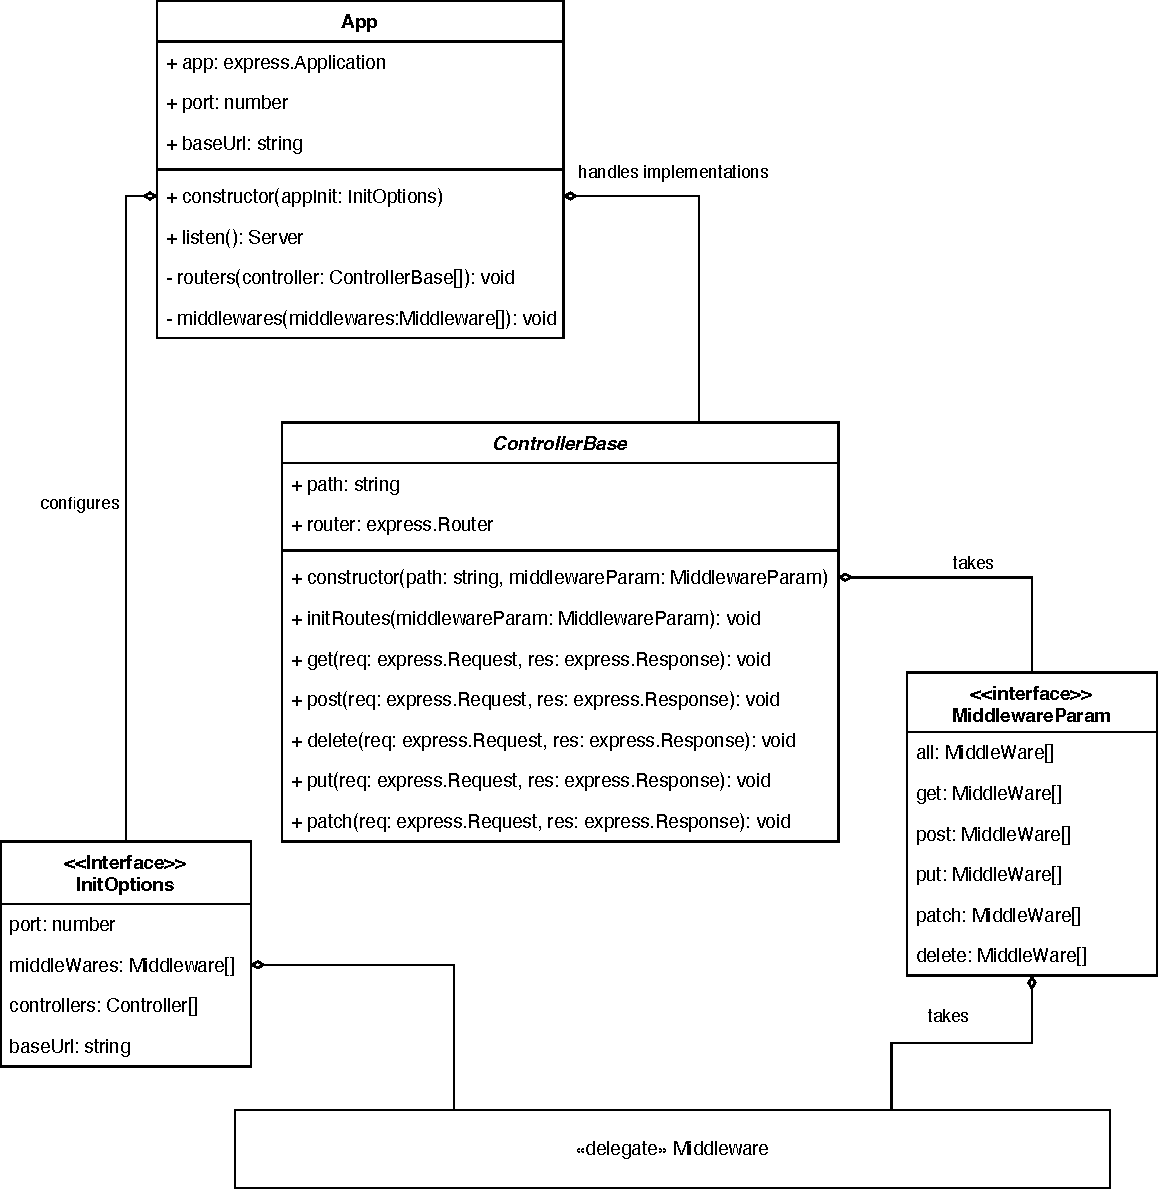
\includegraphics[width=\textwidth]{media/APITemplate/apiArchitecture.svg.pdf}
    \caption{UML Diagramm der API-Architektur}
    \label{fig:apiUML}
\end{figure}

\pagebreak

\hfour{Der "App"-Konstruktor}\label{sec:appConstructor}

Im Konstruktor der App-Klasse können verschiedene Optionen mitgegeben werden:

\hfive{"Port"}

Durch die Port-Option kann angegeben werden, auf welchem Port die API HTTP-Requests annehmen soll. Standardmäßig ist dies auf die Umgebungsvariable "PORT" gesetzt. Die Umgebungsvariablen werden aus einer ".env"-Datei ausgelesen (siehe Seite \pageref{par:dockerEnvFile}). Falls diese nicht gesetzt ist, wird der Port 3000 verwendet.

\hfive{"Controllers"}

Die "Controller" werden als Array von "Controller"-Objekten übergeben und repräsentieren einen Endpunkt (siehe Kapitel "Controllers" \ref{sec:controller}, S. \pageref{sec:controller}).

\hfive{"Middlewares"}

Dies ist ein Array an "Middlewares", welche bei jedem Request vor den "Controllern" ausgeführt werden (siehe Kapitel "Middleware" \ref{sec:middleware}, S. \pageref{sec:middleware}).

\hfive{"Base-URL"}

Durch diesen String kann der Root-Pfad definiert werden. Standardmäßig ist dieser auf "{\ttfamily /}" gesetzt. Bei \ZELIA\ ist dieser auf "{\ttfamily /api}" konfiguriert worden, da alle API bezogenen Anfragen auf den Pfad "{\ttfamily /api}" gehen.

\hfour{Verwendung der APP-Klasse}\label{sec:appUsage}

Um eine Instanz der App-Klasse zu erstellen, muss diese importiert werden. Danach kann die "App" mit ihren registrierten "Controllern" und "Middlewares" instanziiert werden. Damit die "App" auf dem angegebenen Port gestartet wird, muss die "listen"-Methode aufgerufen werden.

\typescript{code/APITemplate/appusage.ts}{Verwendung der App-Klasse}
\hthree{Types}

Das "Types"-Verzeichnis enthält die Interfaces und abstrakten Klassen, wie die "ControllerBase" die benötigt werden, um diesen ExpressJs Wrapper zu nutzen.

\hthree{Die "ControllerBase"-Klasse}

Die abstrakte "ControllerBase"-Klasse ist die Basisklasse eines jeden "Controllers" und stellt die grundlegenden Funktionen bereit. 

Der Konstruktor der "ControllerBase" nimmt zwei Parameter entgegen:

\begin{description}
    \item["path"] Der Pfad, unter dem der "Controller" registriert werden soll.
    \item["middlewareParam"] Ein Objekt, welches das Interface "MiddlewareParam" implementiert und dabei die folgenden Parameter enthält:
    \begin{description}
        \item["all"] Wird bei allen Requests aufgerufen
        \item["get"] Wird bei GET-Requests aufgerufen
        \item["post"] Wird bei POST-Requests aufgerufen
        \item["put"] Wird bei PUT-Requests aufgerufen
        \item["patch"] Wird bei PATCH-Requests aufgerufen
        \item["delete"] Wird bei DELETE-Requests aufgerufen
    \end{description}
\end{description}

\typescript{code/APITemplate/MiddlewareParam.ts}{Interface "MiddlewareParam"}

"Middlewares" sind im Kapitel \ref{sec:middleware} auf Seite \pageref{sec:middleware} beschrieben.

Der Zusammenhang zwischen der "App"-Klasse und der "ControllerBase"-Klasse ist in der Abbildung \ref{fig:apiUML} auf Seite \pageref{fig:apiUML} dargestellt.

\typescript{code/APITemplate/ControllerBase.ts}{"ControllerBase"-Klasse}

\hthree{Controller}

Ein Controller behandelt alle "Requests" auf einem Pfad. 
Controller sind Klassen, welche von der "ControllerBase" erben. Im Super-Konstruktor des Controllers muss der Pfad der Requests angegeben werden, welche vom Controller verarbeitet werden sollen. Zusätzlich kann ein Objekt mit zusätzlichen Middlewares übergeben werden. Um eine HTTP-Methode zu implementieren, müssen lediglich die Methoden "get", "post", "put", "patch" oder "delete" überschrieben werden. Diese nehmen die von "ExpressJS" bekannten Parameter "Request" und "Response". 

\hthree{"Middleware"}\label{sec:middleware}

Bei ZELIA ist eine "Middleware" eine Funktion, die eine bestimmte Signatur hat (siehe Code \ref{code:middlewareSignature}), welche von "express" vor der Handler-Methode des "Controllers" aufgerufen wird. 
Diese benötigt die aus dem NPM-Modul "express" bekannten Parameter:

\begin{itemize}
    \item \textbf{Request-Objekt} ({\ttfamily req}) - beinhaltet alle Informationen des Requests. Dazu zählen \zb\ die Header, Query-Parameter oder der Body.
    \item \textbf{Response-Objekt} ({\ttfamily res}) - ermöglicht das Erstellen einer Antwort. Dafür können mit diesem Objekt der Statuscode, die Header und der Body gesetzt werden.
    \item \textbf{Next-Funktion} ({\ttfamily next}) - muss aufgerufen werden, wenn die Middleware fertig ist, ohne dass dieser die Anfrage durch eine Antwort beendet hat.
\end{itemize}

"Middlewares" können entweder für einzelne Methoden im "Controller", für einzelne "Controller" oder für die gesamte API registriert werden. Soll die Middleware für die gesamte API zur Verfügung stehen, muss diese im App-Konstruktor registriert werden.

\typescript[code:middlewareSignature]{code/APITemplate/middleware.ts}{Signatur einer Middleware}

\hfour{Anwendungsfälle}

Eine "Middleware" könnte zum Beispiel Informationen über die eingehenden "Requests" loggen, damit die Entwickler leichter debuggen können. 
Dabei wird sie im \linebreak App-Konstruktor registriert, um bei jeder Anfrage mitzuloggen. 

\begin{figure}[H]
    \centering
    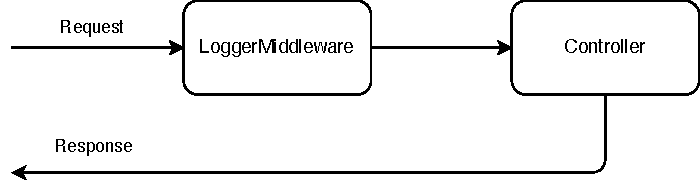
\includegraphics{media/APITemplate/LogMiddleware.svg.pdf}
    \caption{Aufrufreihenfolge der "Middlewares" vor dem "Controller" anhand der "LoggerMiddleware"} 
\end{figure}

\typescript{code/APITemplate/loggerMiddleware.ts}{Beispiel der "LoggerMiddleware"}

"Middlewares" können auch benutzt werden, um den Benutzer beim "Request" zu \mbox{authentifizieren}. 
Dabei wird in der "Middleware" geprüft, ob der Nutzer auf diesen Endpunkt zugreifen darf. Wenn ja, wird die "Next"-Funktion aufgerufen, um die nächste "Middleware" bzw. die Handler-Methode des "Controllers" aufzurufen. Wenn nicht, wird mittels des "Response"-Objektes eine "Unauthorised-Response" geschickt.

Wenn die "Logger"-"Middleware" in der App-Klasse und die "Authentication"-"Middleware" in einem "Controller" registriert sind, wird bei einer Anfrage auf diesen "Controller" zunächst die "Logger"-"Middleware" ausgeführt. Danach wird in der "Authentication"-"Middleware" geprüft, ob der Nutzer berechtigt ist, auf diesen Endpunkt zuzugreifen. Wenn ja, wird die "Next"-Funktion aufgerufen, um die nächste "Middleware" bzw. die Handler-Methode des "Controllers" aufzurufen. Wenn nicht, wird mittels des "Response"-Objektes eine "Unauthorised-Response" geschickt (siehe Abbildung \ref{fig:authMiddleware}).

\begin{figure}[H]
    \centering
    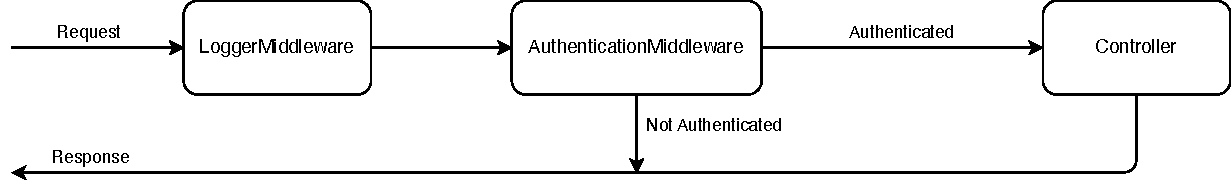
\includegraphics[width=15cm]{media/APITemplate/AuthMiddleware.svg.pdf}
    \caption{Aufrufreihenfolge der "Middlewares" vor dem "Controller" anhand der "LoggerMiddleware" und der "AuthenticationMiddleware" } 
    \label{fig:authMiddleware}
\end{figure}

\typescript{code/APITemplate/authenticationMiddleware.ts}{Beispiel der "Authentication"-"Middleware" }

\htwo{Models}
\htwo{Services}
\htwo{Data}

